% -----------------------------------------------------------------------------------
%                               BIBLIOGRAPHY - Insert Name of BIB File Here
% -----------------------------------------------------------------------------------
\newpage

% ---------------BIBTEX OLD-----------------------------------------------------
% \bibliographystyle{unsrt} %%%% Plain or alpha can change orders here
% \bibliography{BibFile}
% \nocite{*} %%%if you want to see all references even those note cited in the text
% -----------------------------------------------------------------------------------

\printbibliography
% -----------------------------------------------------------------------------------
%                                  APENDIX
% -----------------------------------------------------------------------------------

% \end{counted} %<<<<<<<<<<<<<<ENDS WORD COUNTER

\newpage
\section{Appendices}

\subsection{Meeting Minutes}

\textbf{Meeting 1: 23rd Jan 2018}

Work Flow:

List of tasks for next 3 weeks compiled:

\textbf{Week 1:} Requirements gathering

\begin{itemize}
  \item Industry Research
  \item Everybody to research how to use Latex
  \item Shared resources to be set up: Github, Latex, One Drive

\end{itemize}


\textbf{Week2:} Refinement of requirements (including categorisation)

\begin{itemize}
  \item MoSCoW prioritisation and effort estimation for requirements
  \item Begin thinking about use cases


\end{itemize}


\textbf{Week 3:} Continue developing use cases

\begin{itemize}
  \item Need to consider who stakeholders for the app are (company, renters of tools).
  \item The application should be designed as a web app – for use in a browser and mobile.
  \item Phoebe to share UML 2.0 book to use for UML syntax / diagrams.
  \item Daiana to act as SCRUM master for project.


\end{itemize}


\textbf{Plan for next meeting}

To meet every Tuesday 11am - 1pm, possibly in room in Foster Court.

Next Meeting to bring post-its (!) to help organise requirements visually.

\textbf{Meeting 2: 30th Jan 2018}



\begin{itemize}
  \item This week focus on use cases and organise requirements.
  \item Brief discussions of Object oriented diagrams, sequence diagrams, activity diagrams
  \item Came up with non-functional requirements for the project
  \item Came up with non-functional requirements for the project
 
\end{itemize}



\textbf{First Meeting with Rae}

Review of vision and scope

Suggested we should convert requirements to excel and number them

She suggested that performance tests run on key functions can help determine non-functional requirements in an actual implementation

\textbf{Meeting 3: 6th Feb 2018}

\textbf{Discussed:}
Actors:

User – anyone that interacts with the system, Customer, Employee, Admin, Customer Support, Credit Card Company, Delivery service, Notification Service, Database

To Do this Week:
\begin{itemize}
  \item Finish writing up Use Cases and make sure they match names on use case diagram
  \item Finish analysis class diagram

\end{itemize}

\textbf{Meeting 4: 13th Feb 2018}

\begin{itemize}
  \item Refining Use-cases
  \item Discussion about state machine diagrams- Rae gave some examples and the group plans to review these
  \item Class diagrams- inclusion of getters and setters
  \item Sequence diagrams- making sure they are consistent with class diagrams


\end{itemize}

\textbf{Meeting 5: 6th March 2018}

\begin{itemize}
	\item Discussion of analysis and design class diagrams final changes- adding JSP/JavaClass notation to design and Boundary, Controller, Entity notation to the analysis class diagrams
	\item Discussion of final modification for sequence diagrams
	\item Clarification about deployment diagrams- modelling how a three tier architecture system would be deployed

\end{itemize}

\textbf{Meeting 6: 15th March 2018}

\begin{itemize}
	\item Final diagrams discussed 
	\item Discussion of report section allocation
	\item Discussion of presentation assembly

\end{itemize}

\textbf{Meeting 7: 20th March 2018}

\begin{itemize}
  \item Final report looked over by Rae: edit the alternative flow of use cases
  \item Making presentation for video and shooting video 

\end{itemize}

\subsection{Design Class Diagram Iterations}


\subsubsection{Iteration One}

\begin{figure}[H]
      \centering
      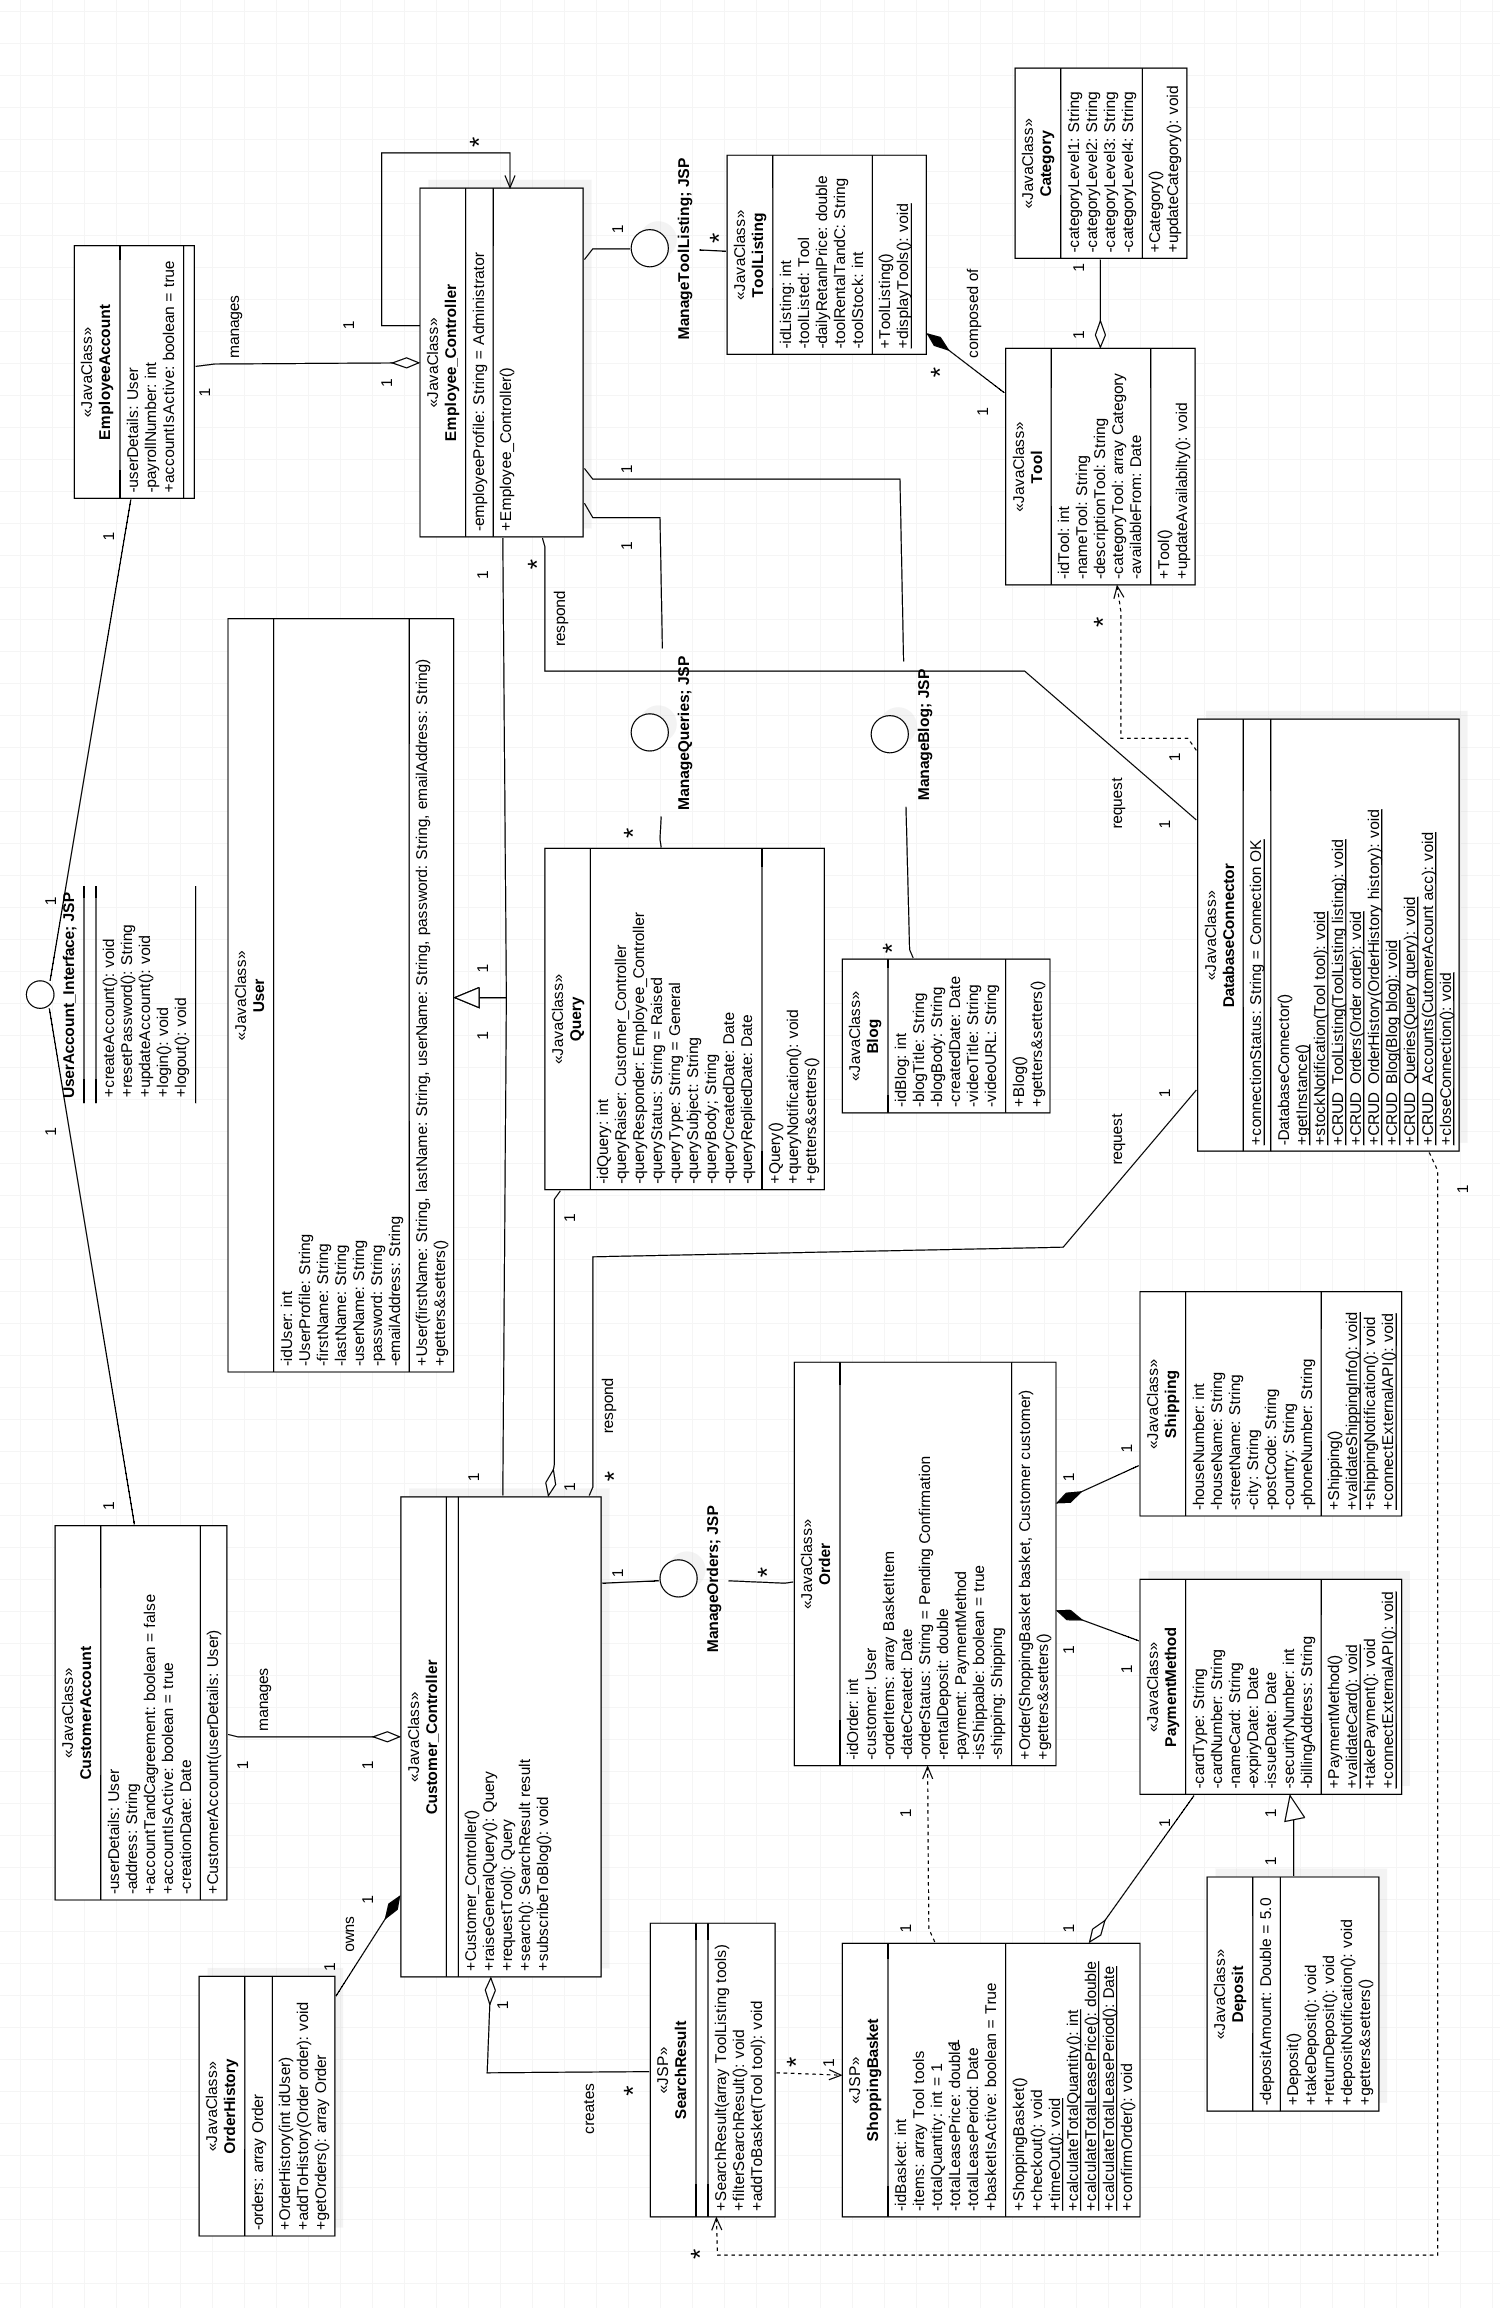
\includegraphics[trim = 0 0 0 0, clip, width=0.7\textwidth]{TempImg/DClass1.png}
      \caption{First iteration of design class diagram}
\end{figure}

\subsubsection{Iteration Two}

\begin{figure}[H]
      \centering
      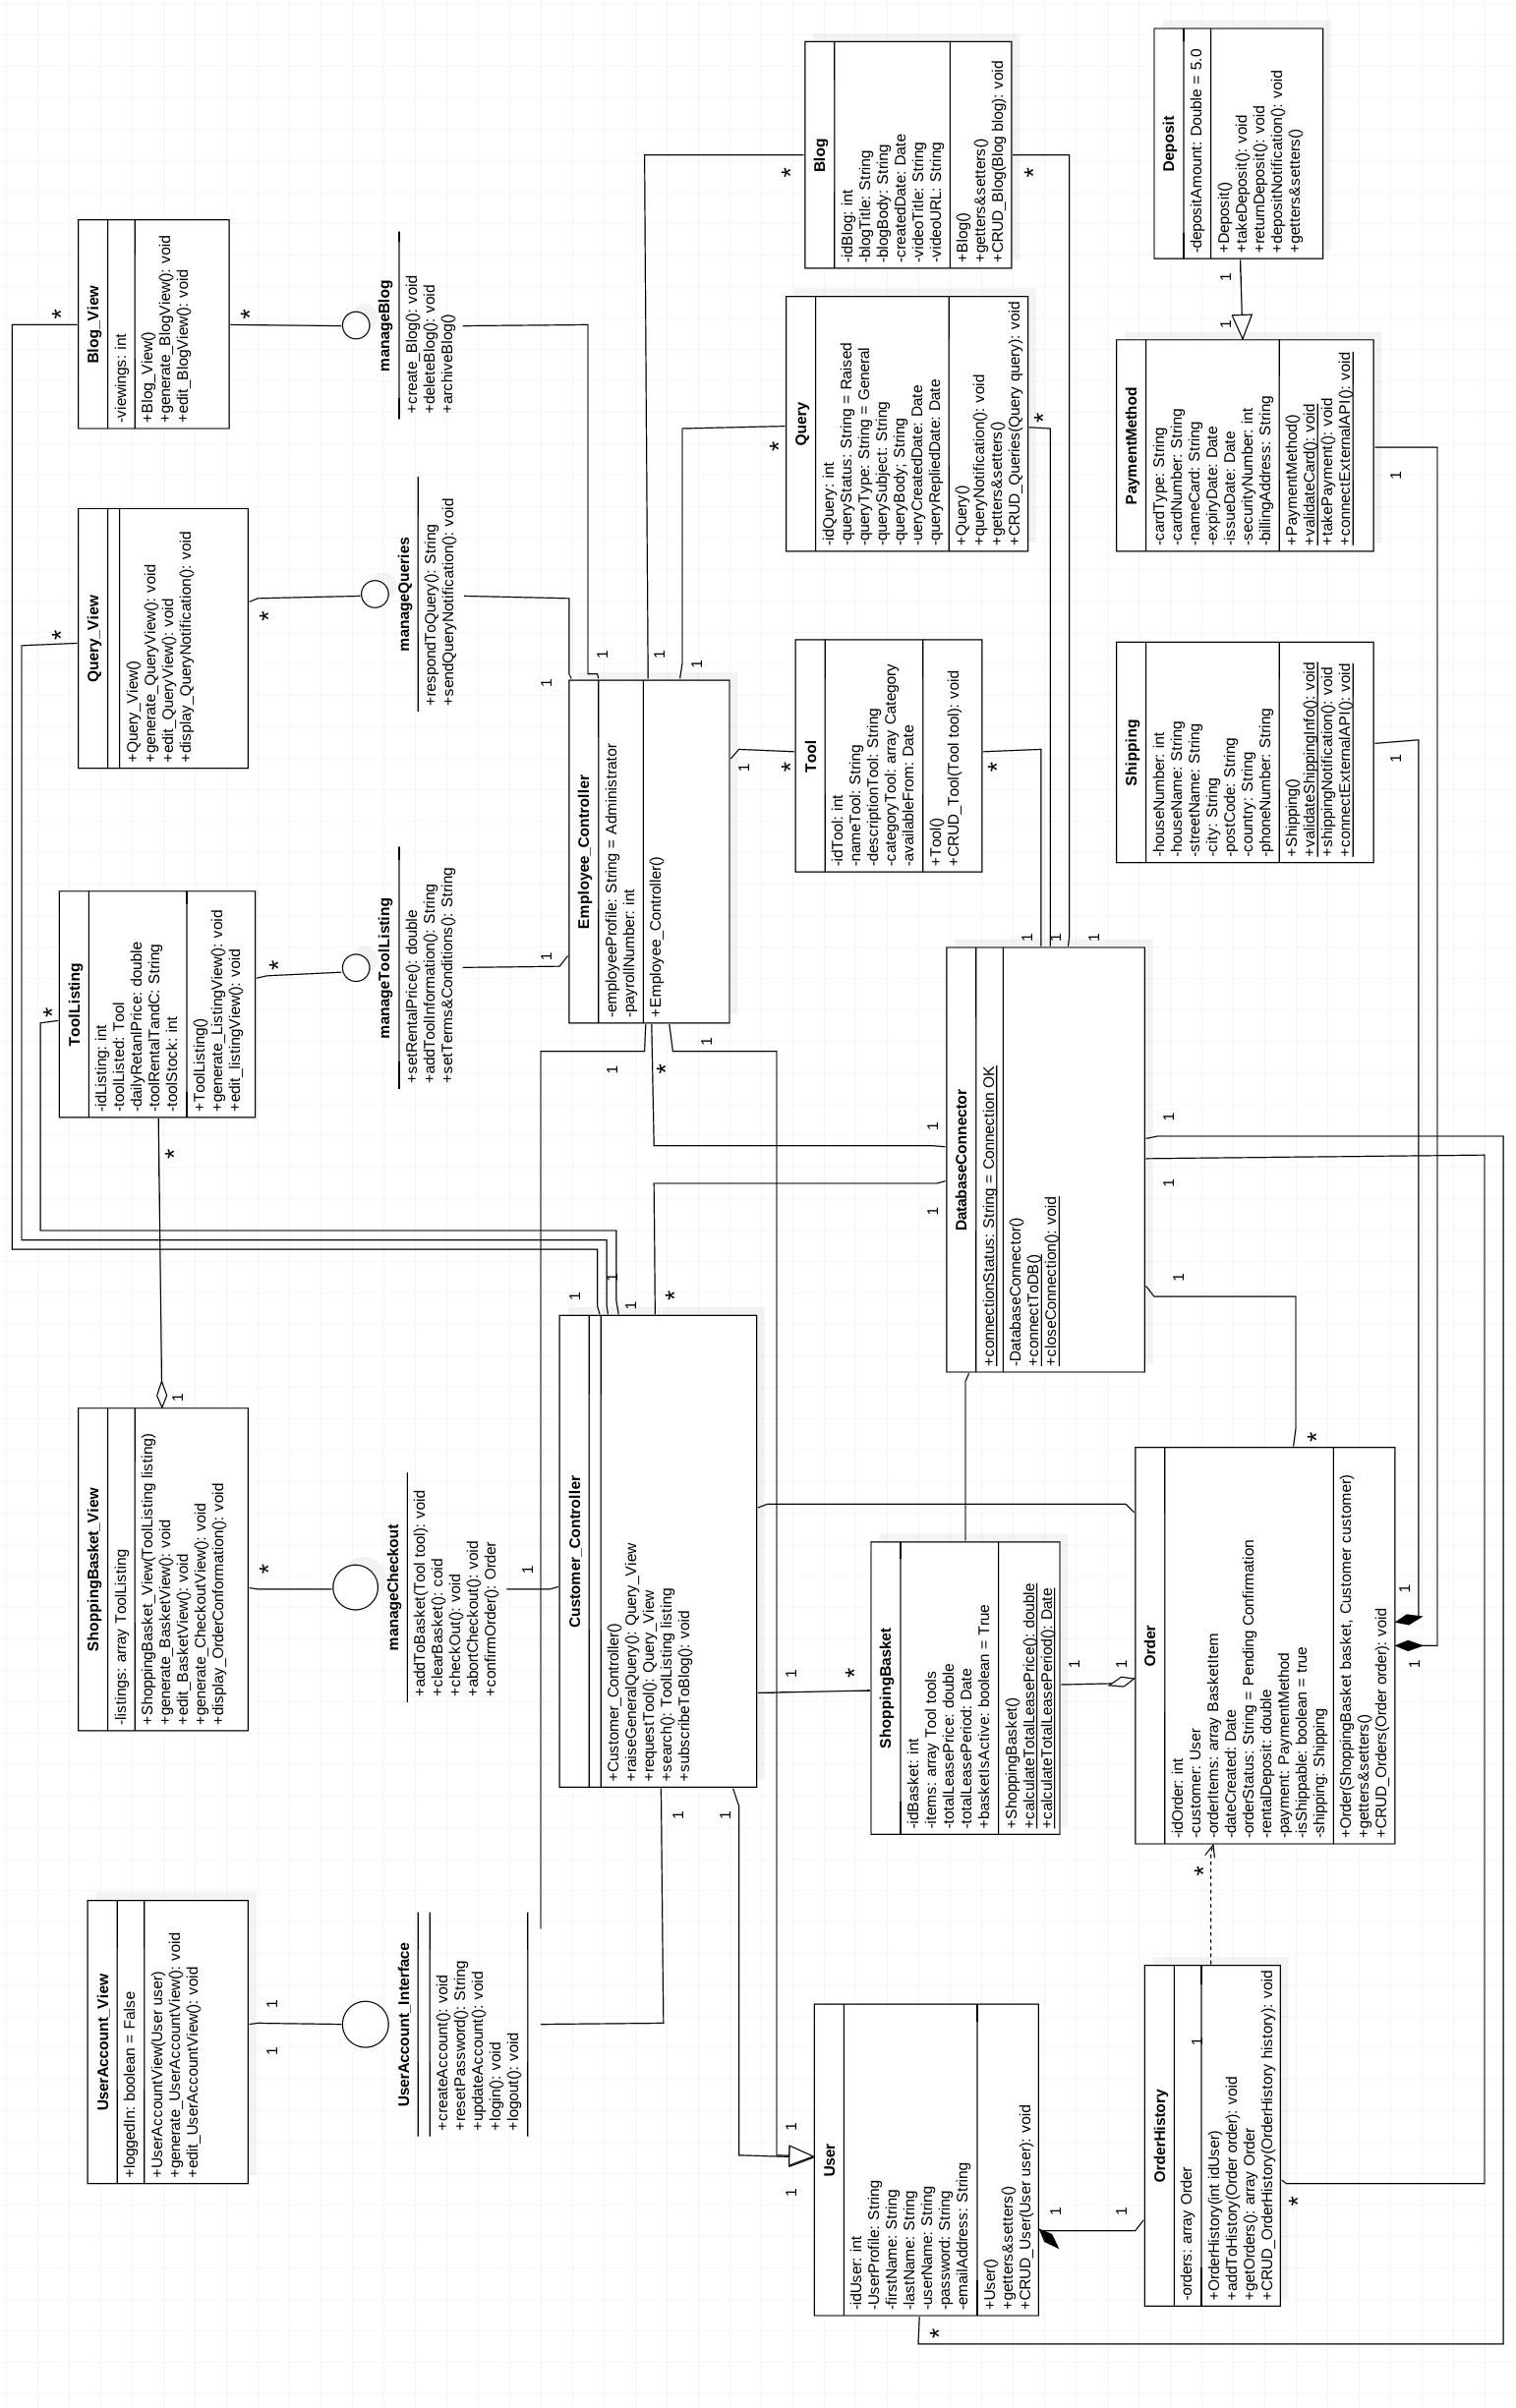
\includegraphics[trim = 0 0 0 0, clip, width=0.75\textwidth]{TempImg/DClass2.png}
      \caption{Second iteration of design class diagram}
\end{figure}


\subsection{Sequence Diagram Iterations}


\subsubsection{Iteration One: Creates Order}

\begin{figure}[H]
      \centering
      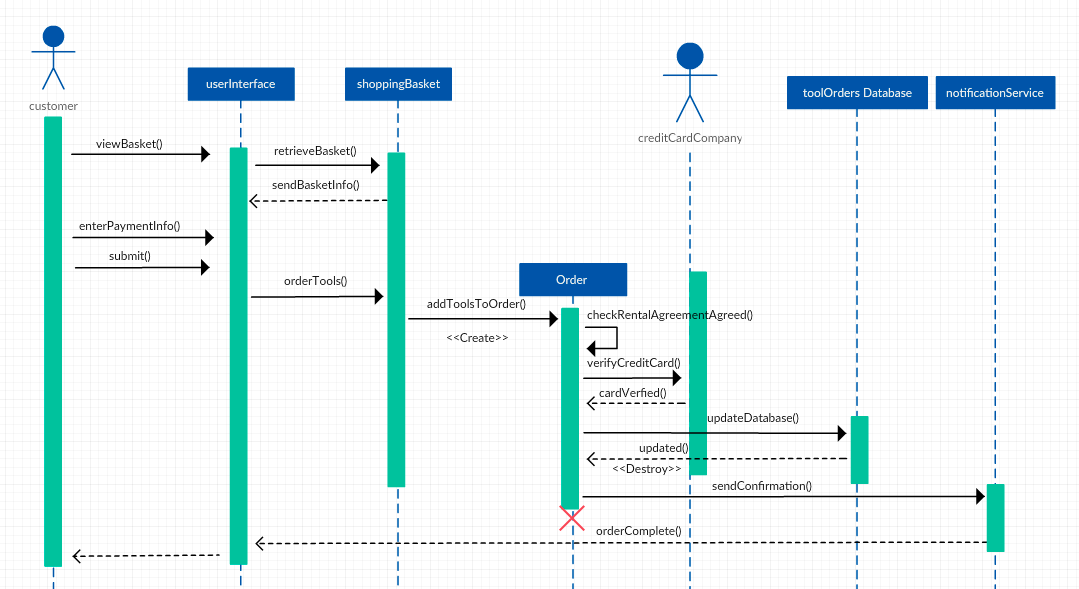
\includegraphics[trim = 0 0 0 0, clip, width=0.8\textwidth]{TempImg/oldSD1_1.png}
      \caption{First iteration of "Creates Order" sequence diagram}
\end{figure}

\subsubsection{Iteration Two: Creates Order}

\begin{figure}[H]
      \centering
      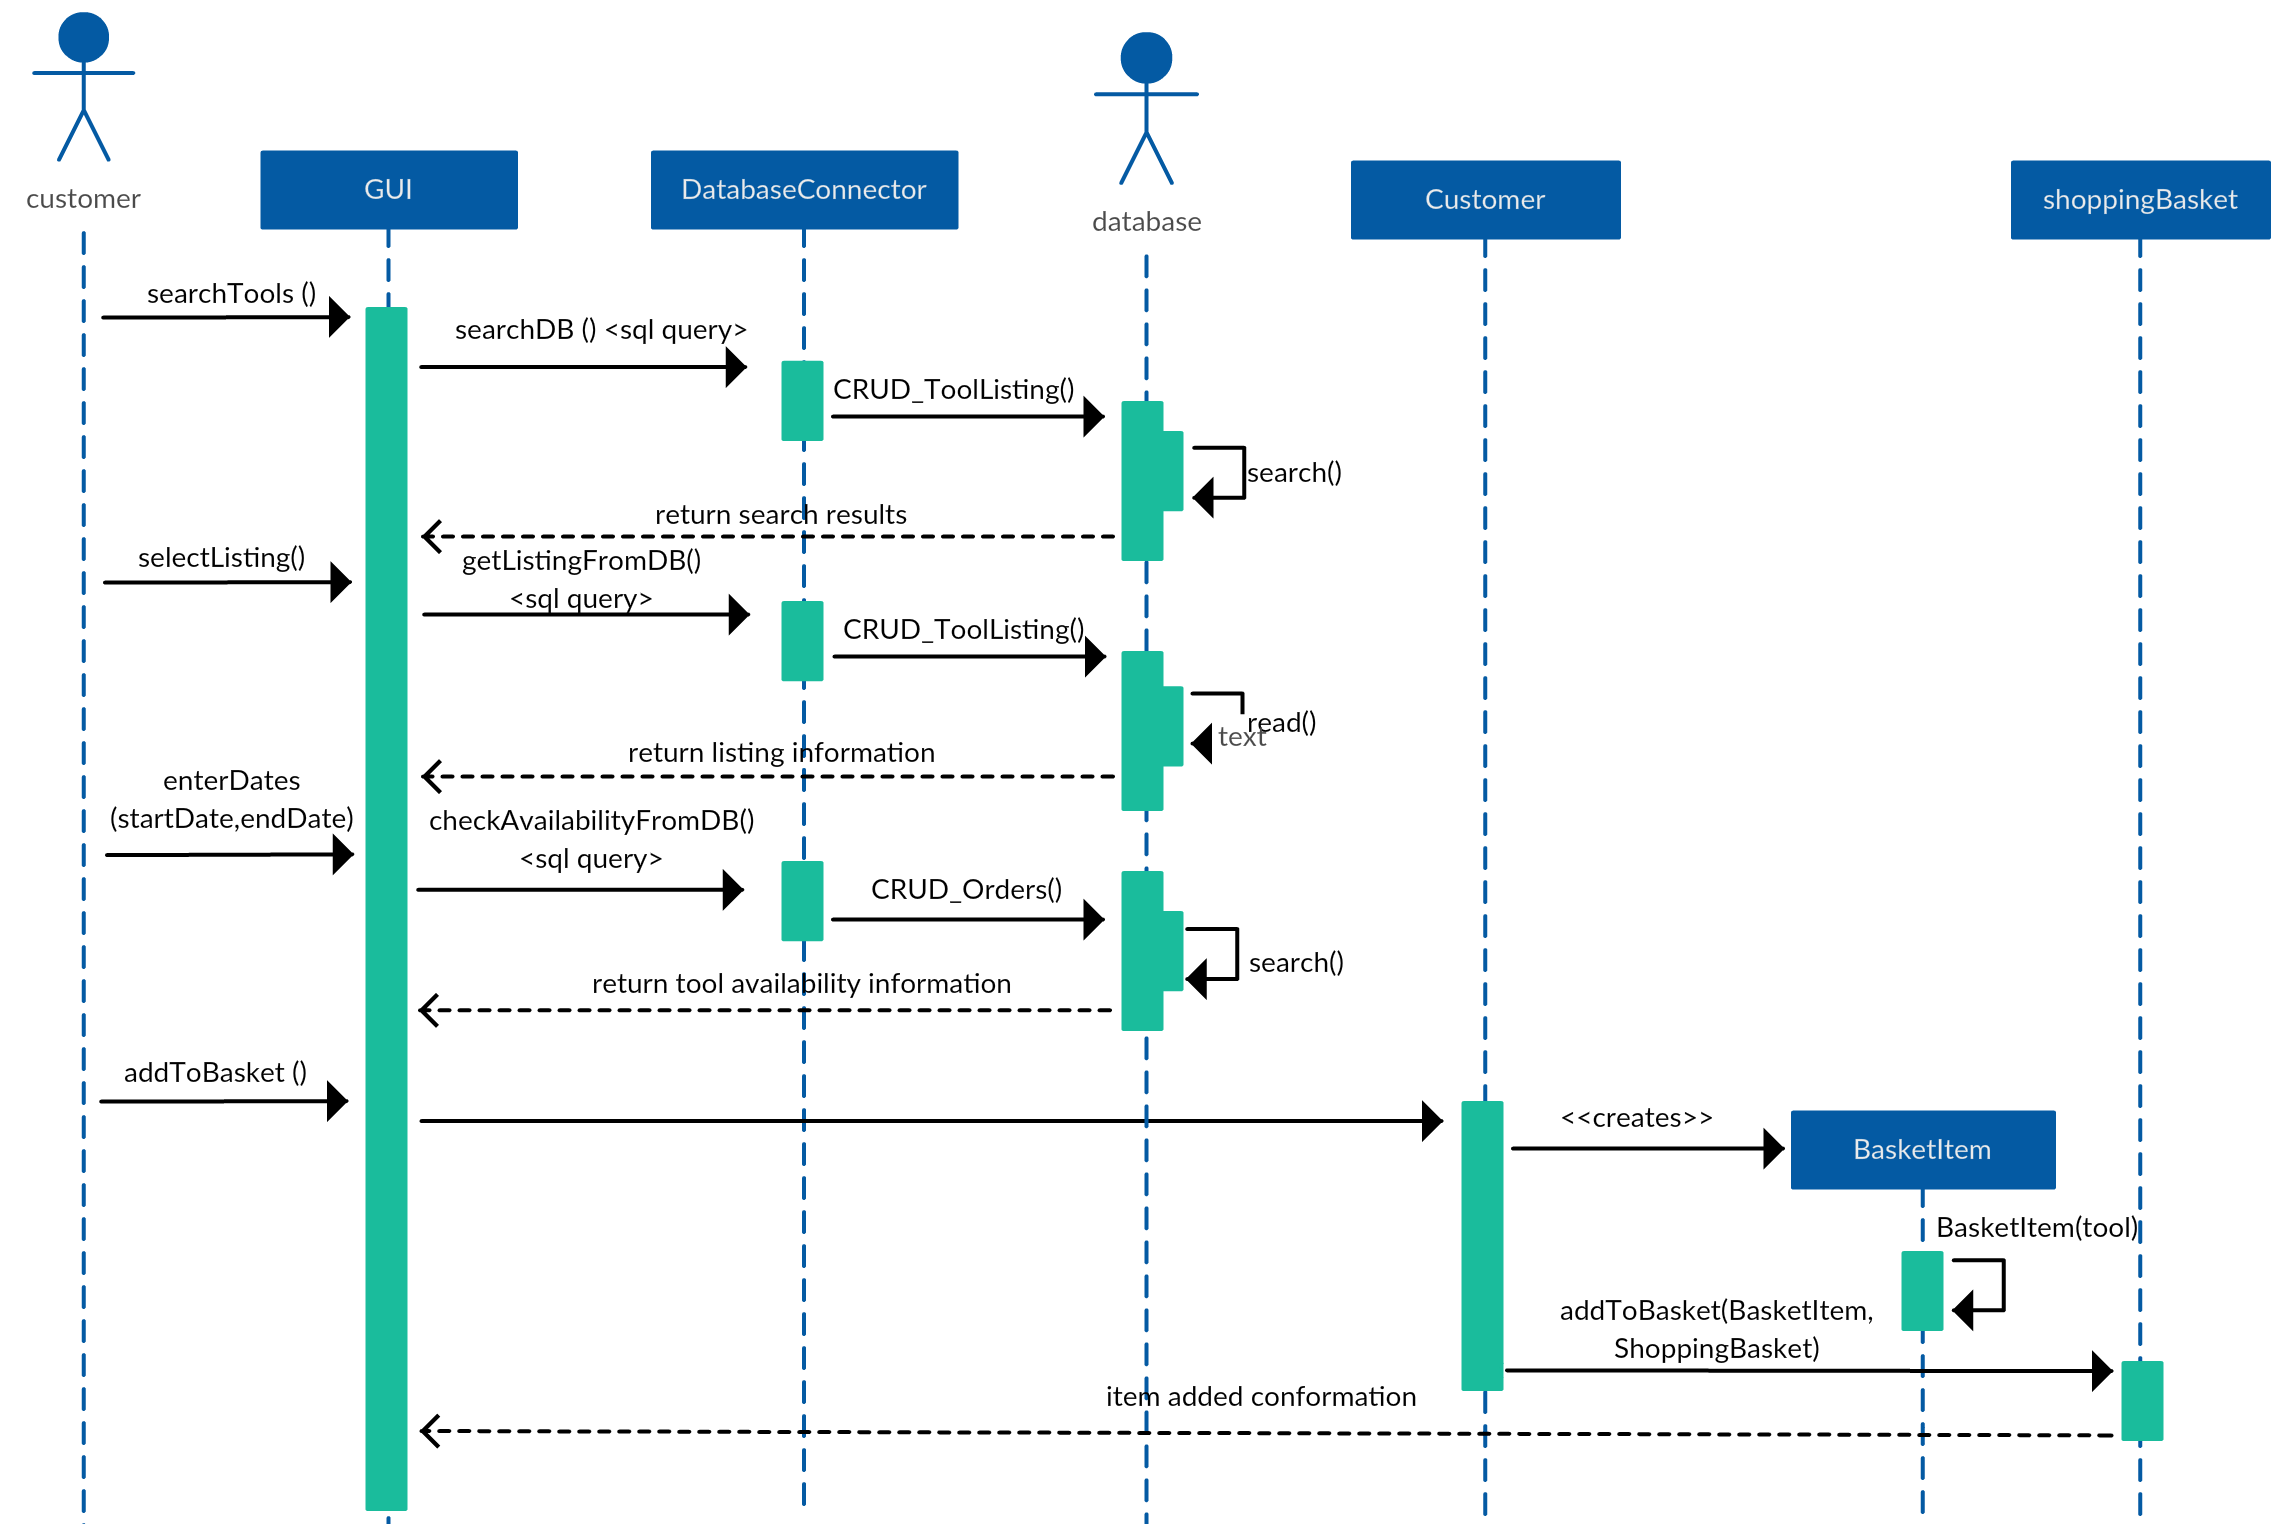
\includegraphics[trim = 0 0 0 0, clip, width=0.8\textwidth]{TempImg/SD1_1.png}
      \caption{Second iteration of "Creates Order" sequence diagram}
\end{figure}

\subsubsection{Iteration One: Checks Out}

\begin{figure}[H]
      \centering
      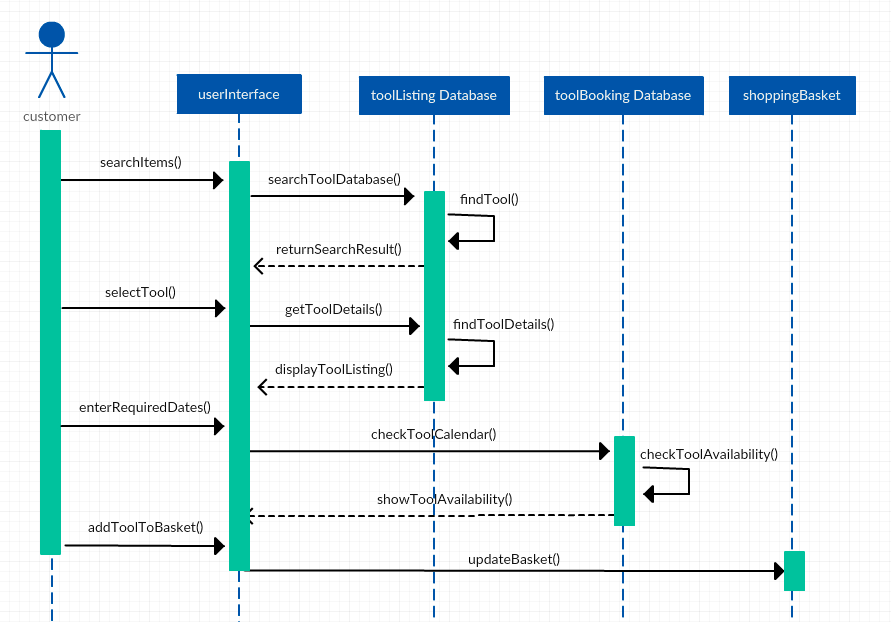
\includegraphics[trim = 0 0 0 0, clip, width=0.8\textwidth]{TempImg/oldSD1_2.png}
      \caption{First iteration of "Checks Out" sequence diagram}
\end{figure}

\subsubsection{Iteration Two: Checks Out}

\begin{figure}[H]
      \centering
      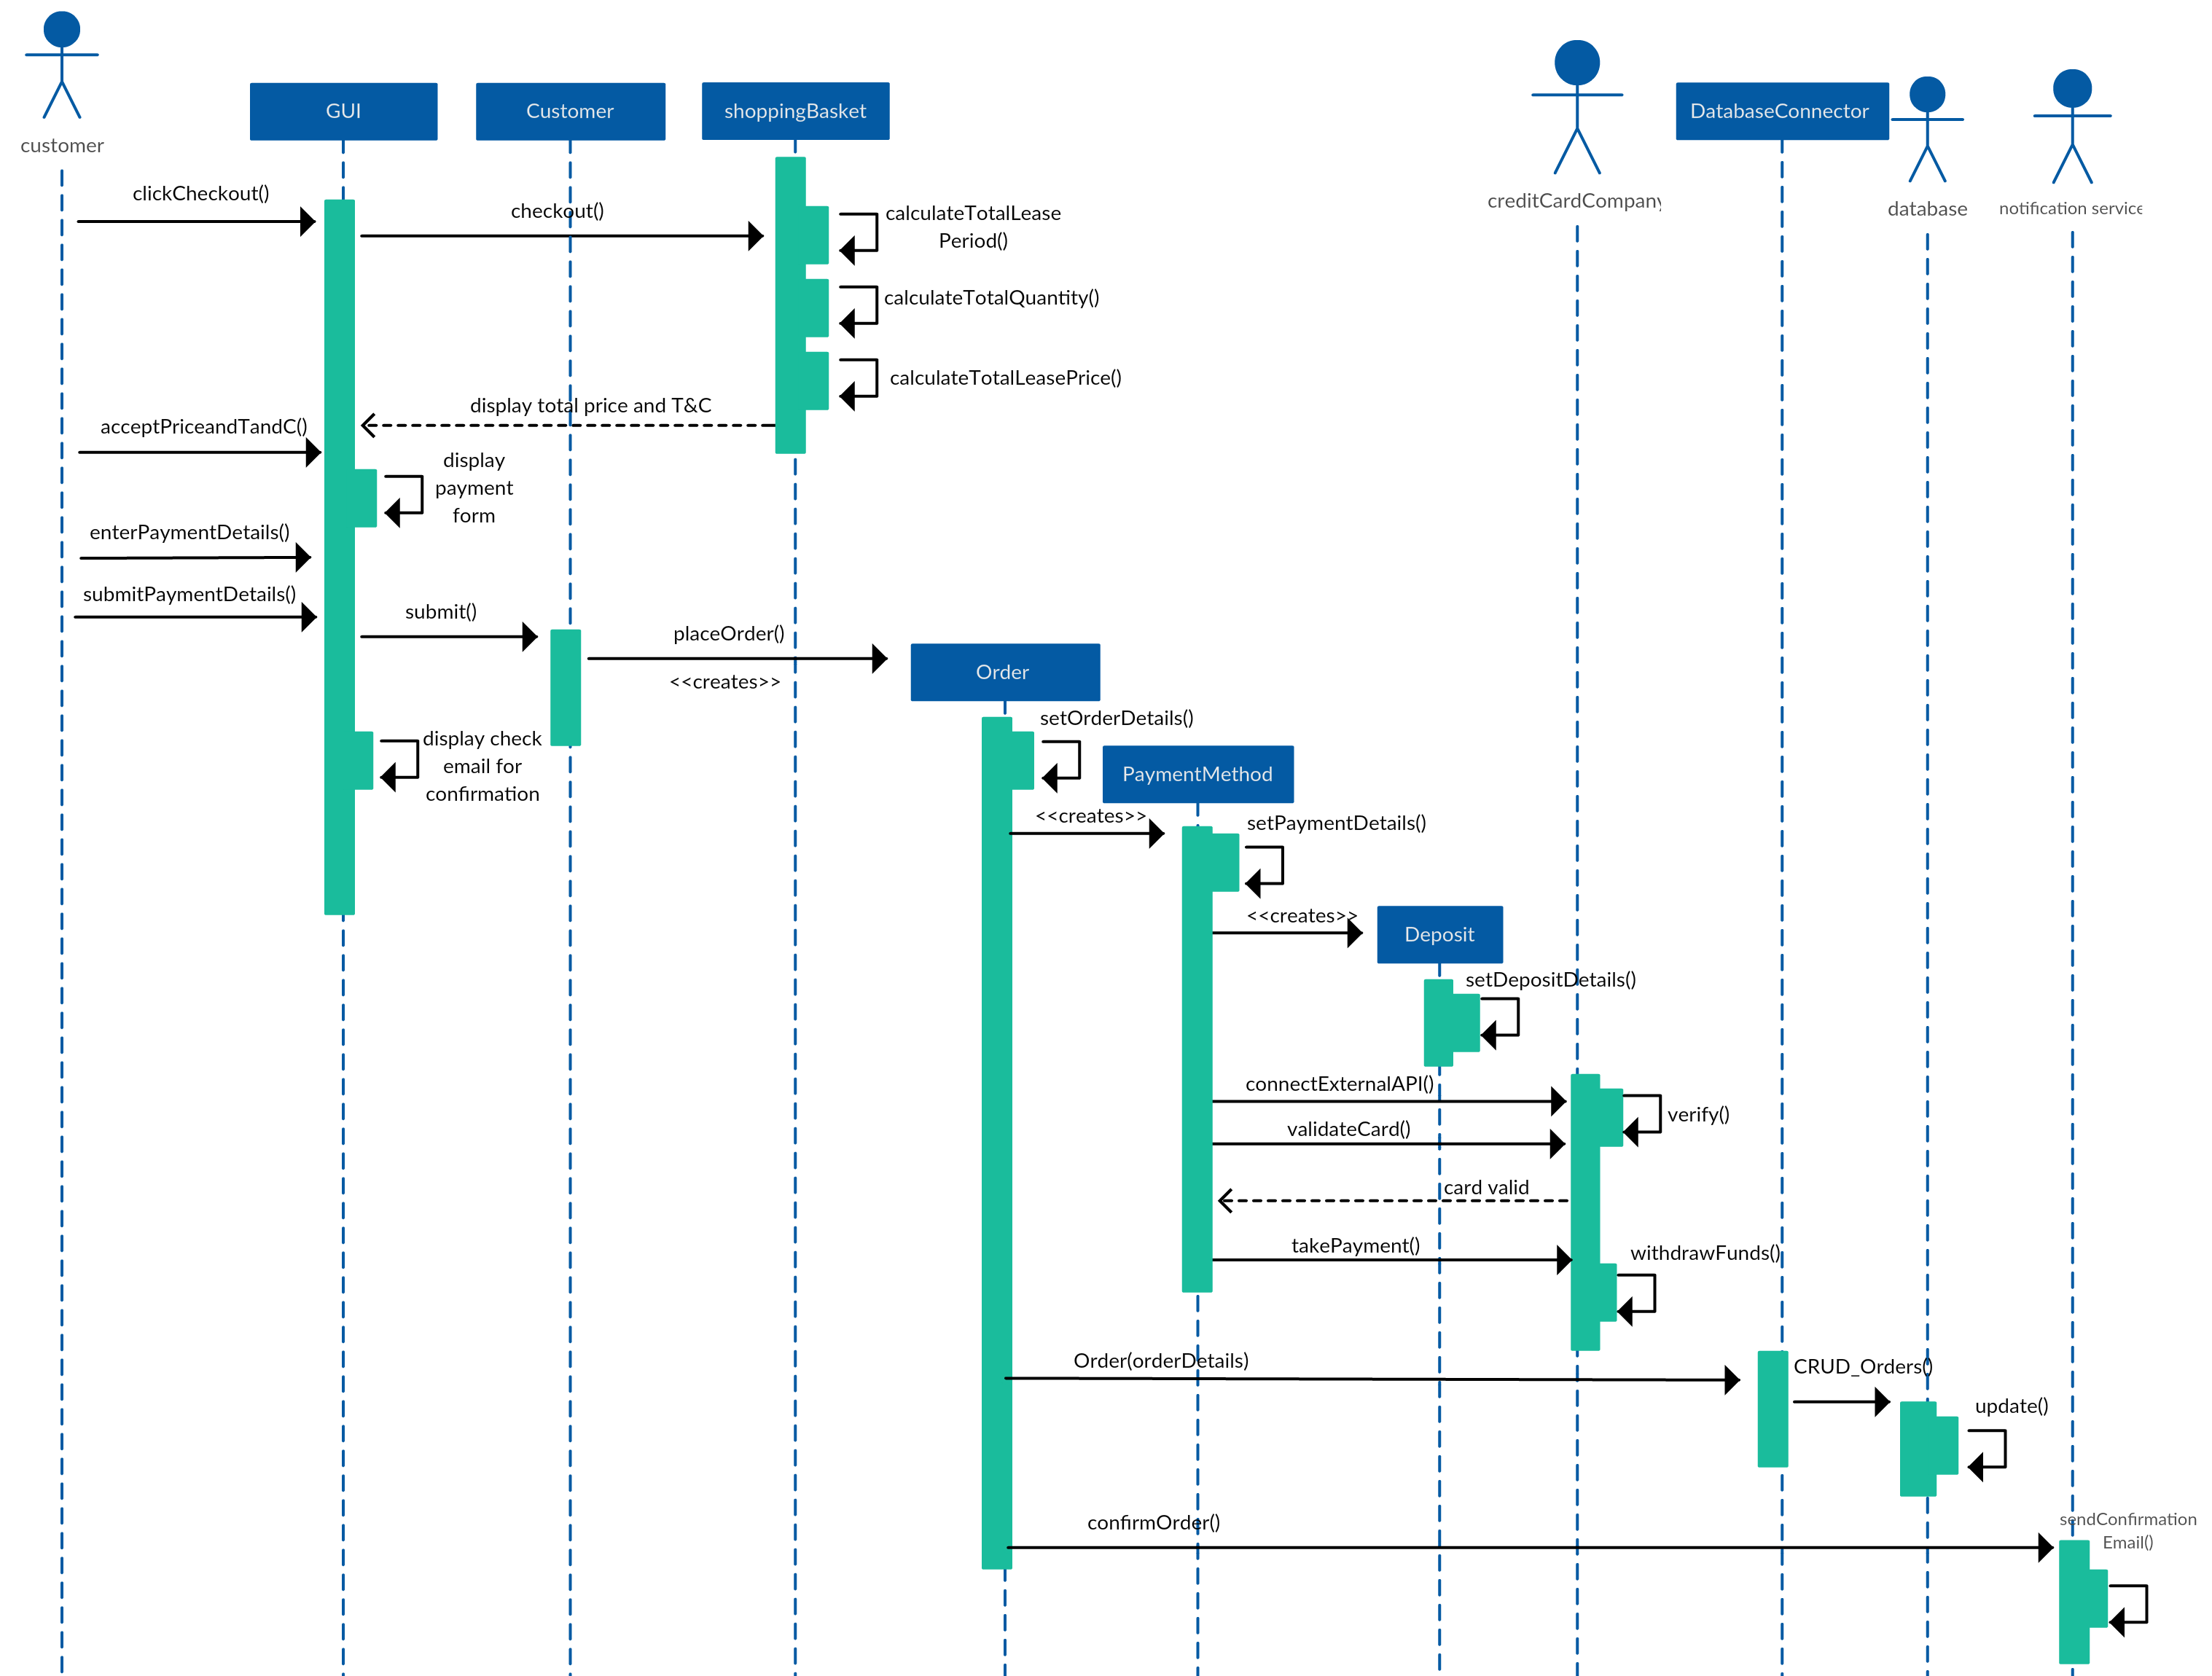
\includegraphics[trim = 0 0 0 0, clip, width=0.8\textwidth]{TempImg/SD1_2.png}
      \caption{Second iteration of "Checks Out" sequence diagram}
\end{figure}

\newpage
\section{Team Member Contribution}

\begin{table}[H]
      \centering
      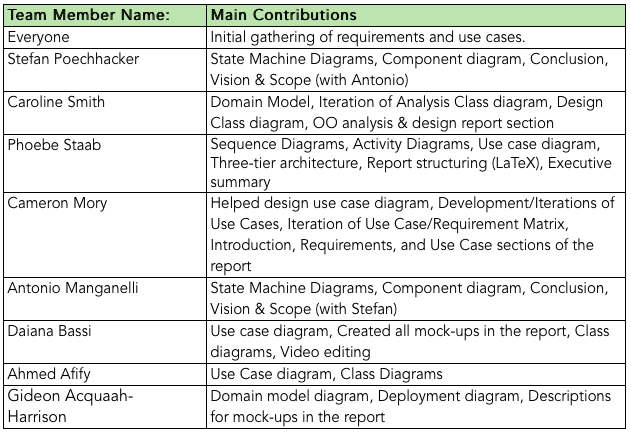
\includegraphics[trim = 0 0 0 0, clip, width=0.7\textwidth]{TempImg/TC.png}
      \caption{Overview of Group A team member contributions}
\end{table}




\end{document}